%!TEX root=../main.tex
\section{More results} % (fold)
\label{sec:more_results}

\begin{figure}
     \centering
    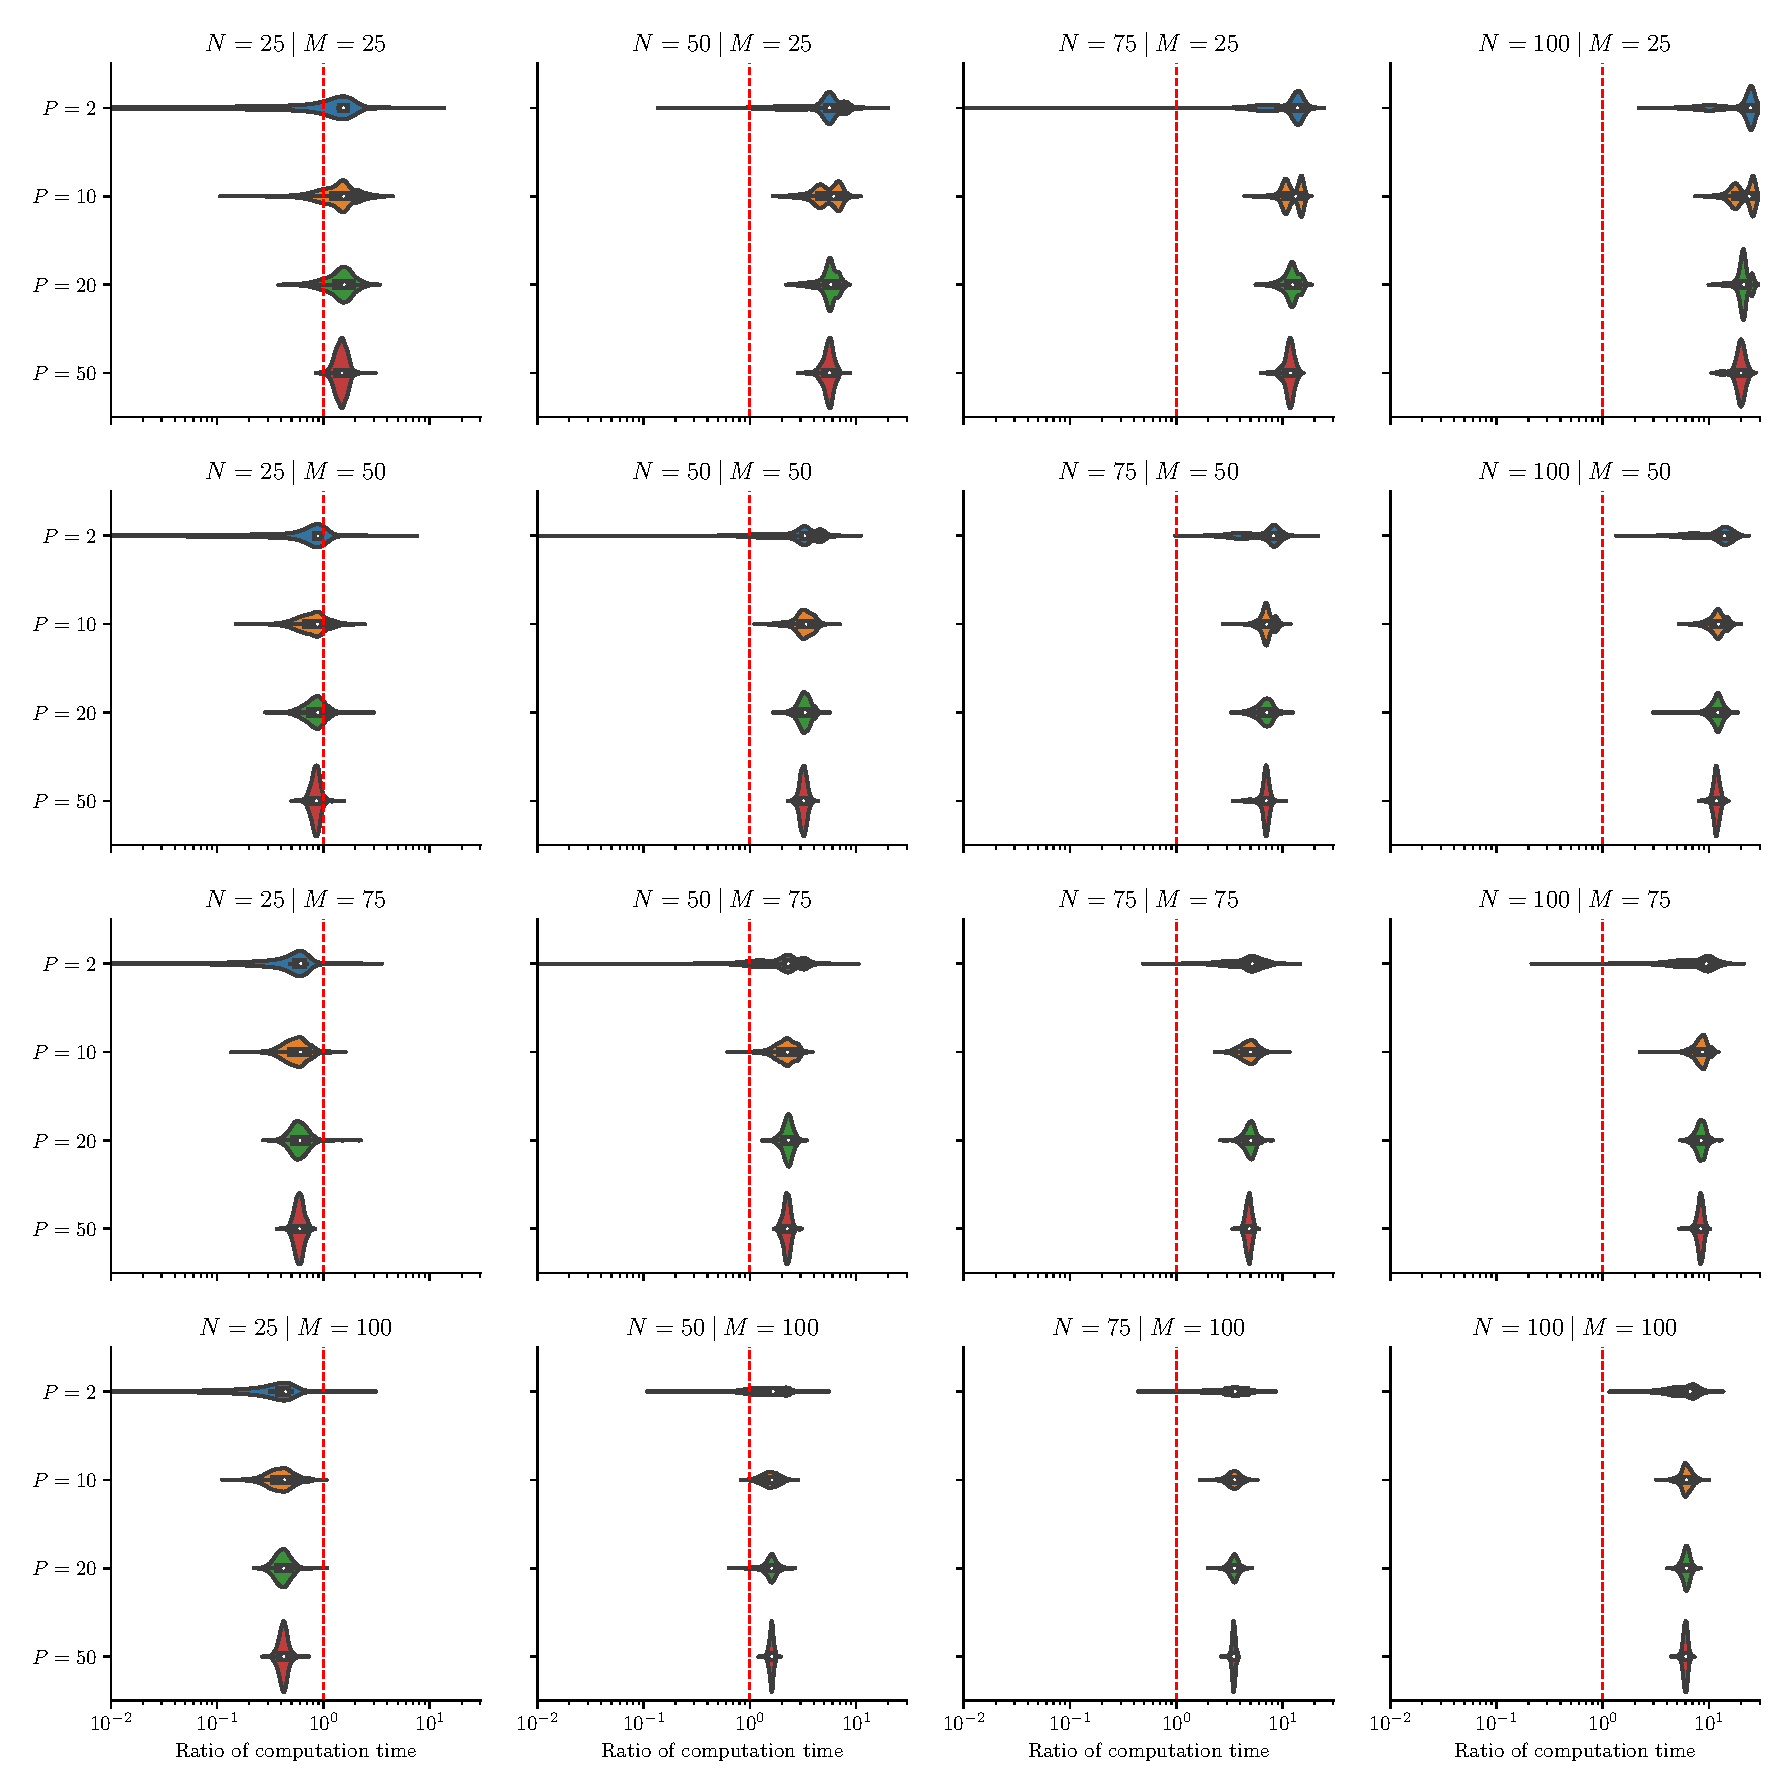
\includegraphics[width=0.95\textwidth]{figures/scenario_1/computation_time.eps}
    \caption{Ratio of computation time for Scenario 1 between the Gram matrix method and the covariance operator method. Each univariate component is defined on a one-dimensional domain. $N$ is the number of observations, $M$ is the number of sampling points per curve and $P$ is the number of features.}
    \label{fig:computation_time_mfd_1d}
\end{figure}

\begin{figure}
     \centering
    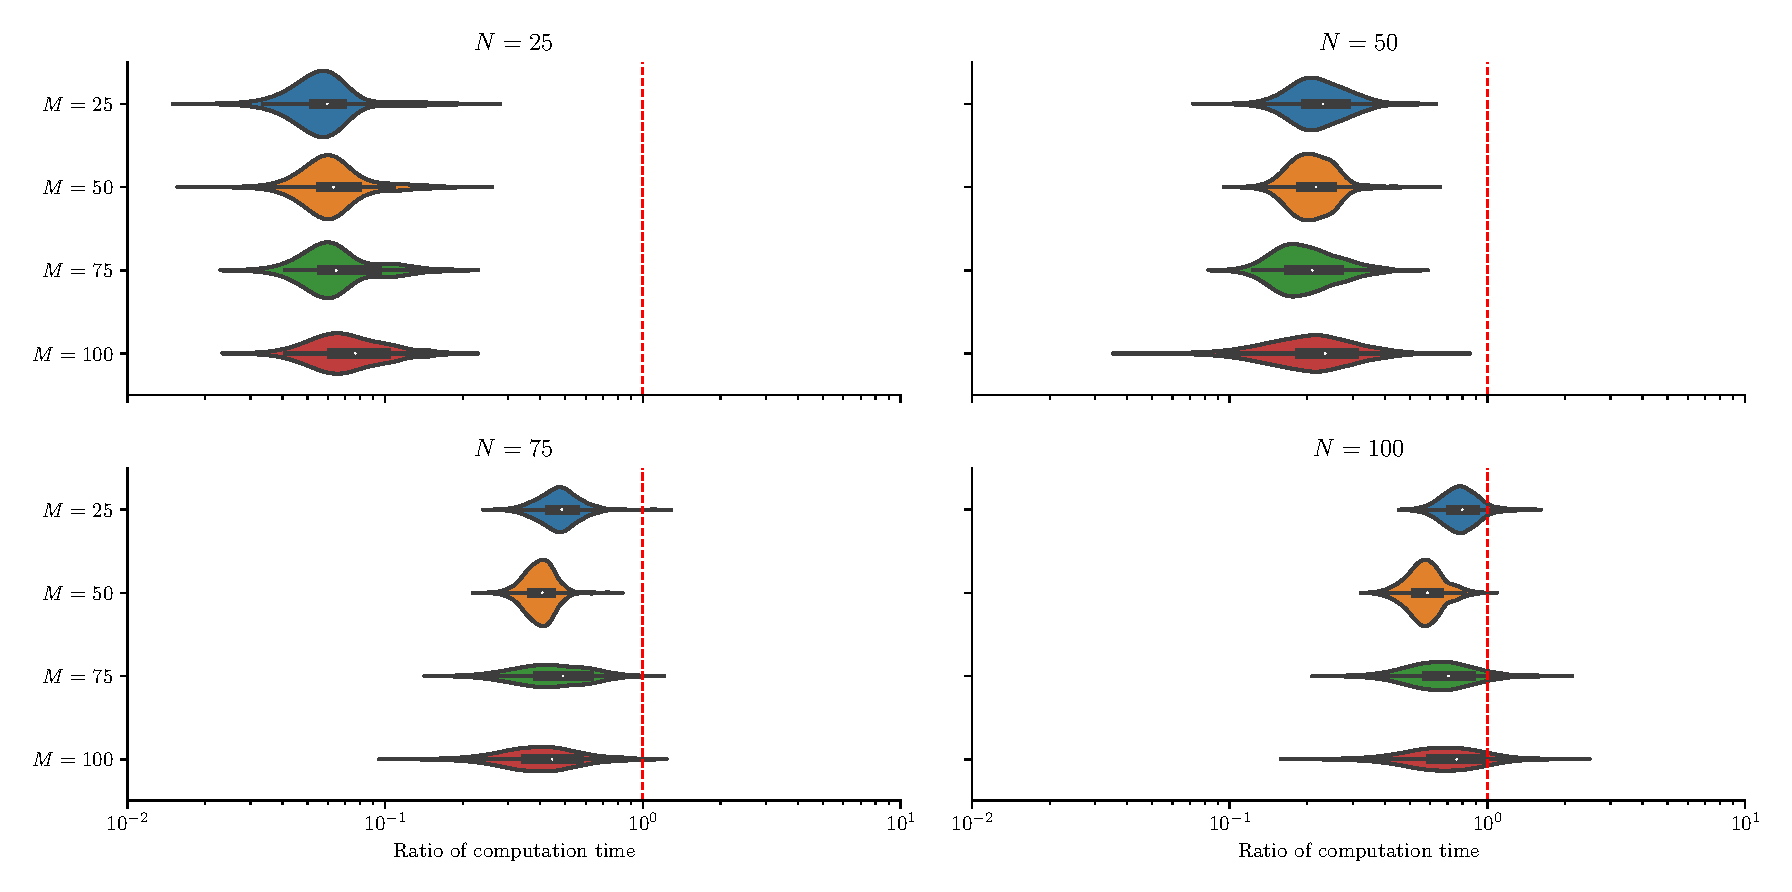
\includegraphics[width=0.95\textwidth]{figures/scenario_2/computation_time.eps}
    \caption{Ratio of computation time for Scenario 2 between the Gram matrix method and the covariance operator method. $N$ is the number of observations and $M \times M$ is the number of sampling points per images.}
    \label{fig:computation_time_mfd_2d}
\end{figure}

\subsection{Simulation} % (fold)
\label{sub:simulation}

% subsection simulation (end)

\subsection{Application} % (fold)
\label{sub:application}

% \begin{figure}
%     \centering
%     \begin{subfigure}[b]{0.45\textwidth}
%         \centering
%         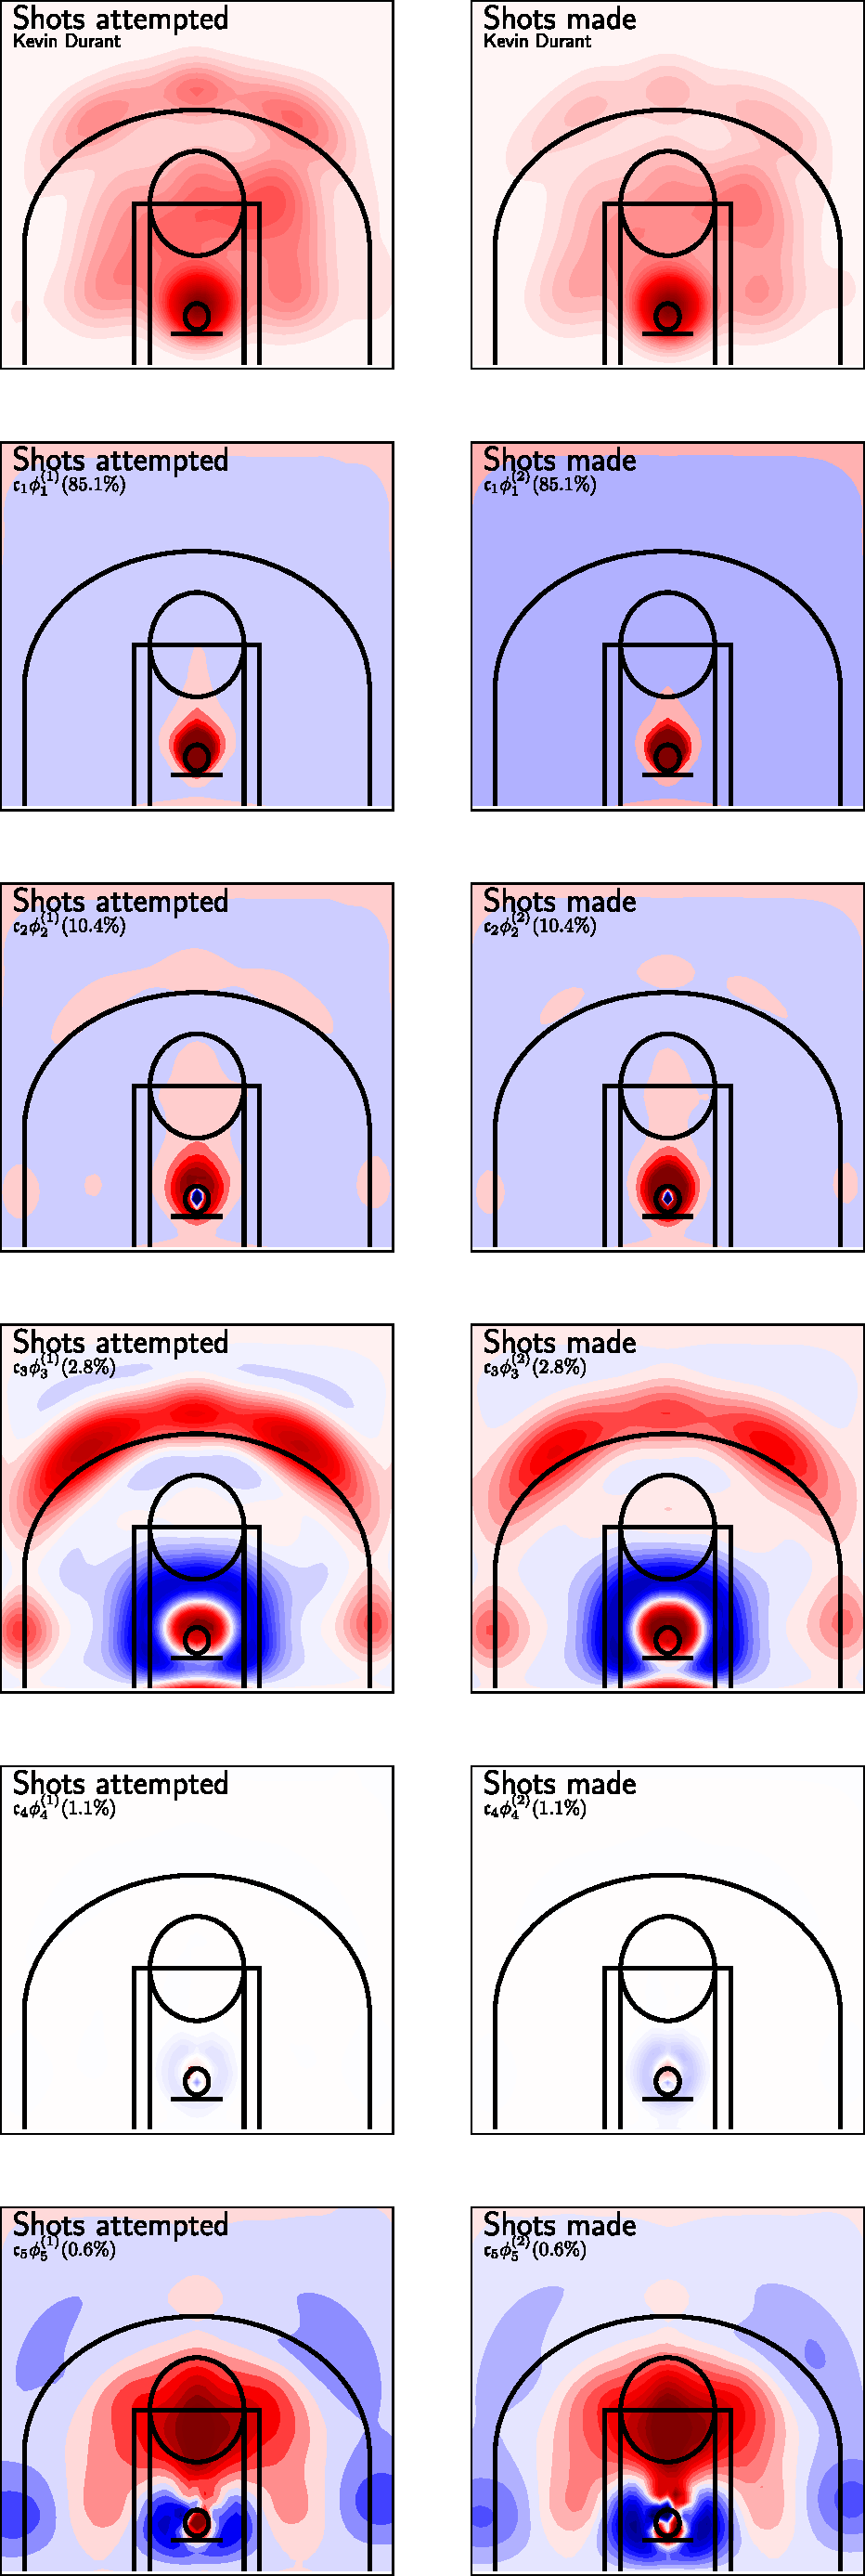
\includegraphics[width=\textwidth]{figures/durant_decomposition.pdf}
%         \caption{Gram matrix}
%         \label{fig:durant_decomposition}
%     \end{subfigure}
%     \hfill
%     \begin{subfigure}[b]{0.45\textwidth}
%         \centering
%         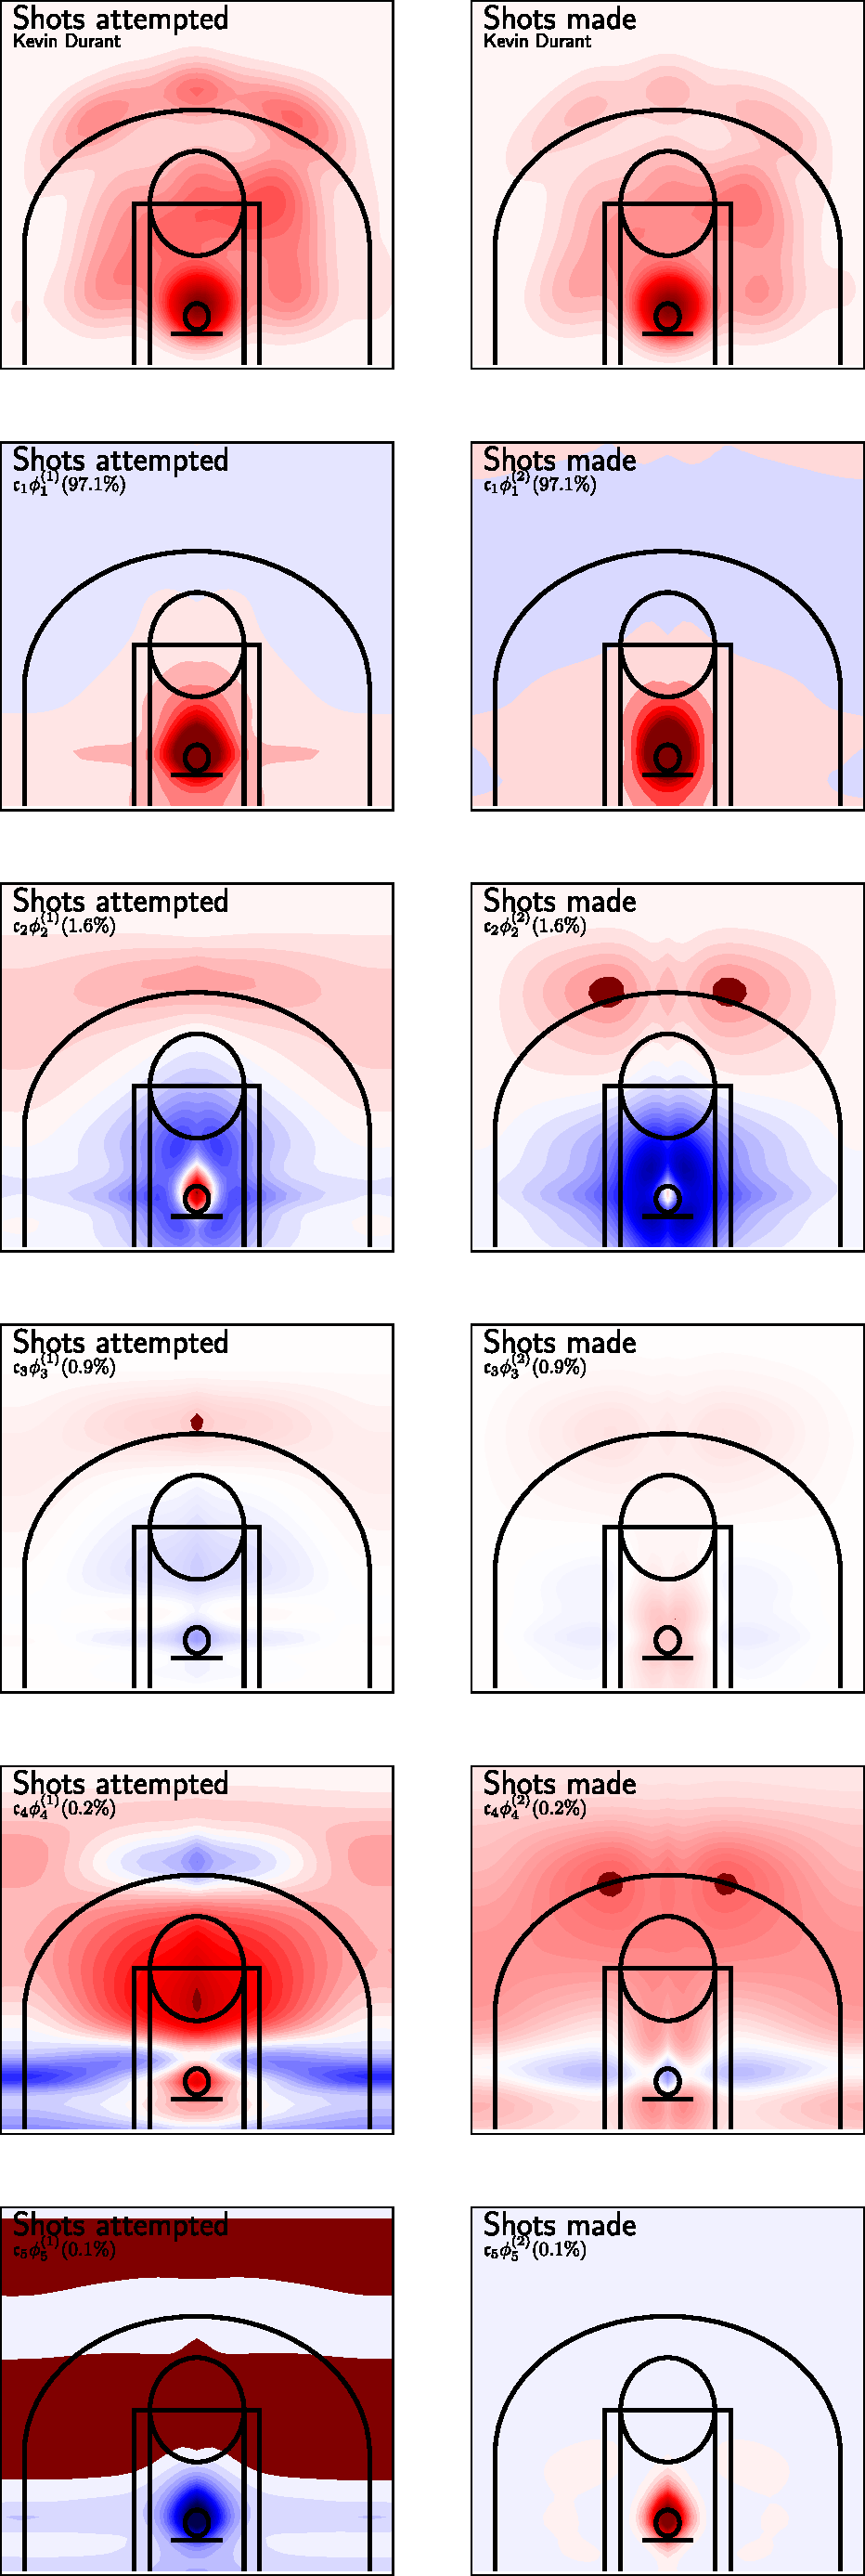
\includegraphics[width=\textwidth]{figures/durant_decomposition_fcptpa.pdf}
%         \caption{FCPTPA}
%         \label{fig:durant_decomposition_fcptpa}
%     \end{subfigure}
%     \caption{Decomposition for Kevin Durant.}
%     \label{fig:durant_shoots_decomposition}
% \end{figure}

% subsection application (end)

% section more_results (end)